\section{Laufzeitanalyse}
\label{laufzeitanalyse}

Die Vorverarbeitung der Eingabedaten sowie das Training der neuronalen Netze erfolgte auf einem 3.5 GHz 6-Core Intel Xeon E5, 16GB DDR3 Arbeitsspeicher und einer Solid-State-Drive.
Die in dieser Arbeit präsentierten Laufzeiten wurden ausschließlich über Berechnungen auf dem Prozessor gewonnen.
Bei der Verwendung einer Grafikkarte stellen sich dabei Laufzeitgewinne in Bereichen, die auf die diese ausgelagert werden können, von $300 - 400 \%$ ein.

\paragraph{Vorverarbeitung}

Die Vorverarbeitung der Eingabedaten in eine geeignete Graphrepräsentation, das Berechnen der Merkmalsmatrix sowie zusätzliche Aufwände wie die Vergröberung des Graphen oder die Bestimmung der Receptive-Fields seiner Knoten, welche für die Eingabe in ein neuronales Netz notwendig sind, trägt einen entscheidenen Anteil an der Ausführungsgeschwindigkeit des Trainings und der Auswertung eines neuronalen Netzes bei.
Graphen sollen dabei bestmöglichst zur Laufzeit eines Trainings generiert werden können und möglichst die Ausführung des eigentlichen Trainings garnicht bis kaum beeinflussen.

Abbildung~\ref{fig:laufzeit_raeumlich_pipeline} illustriert die relative Laufzeitverteilung der einzelnen räumlichen Vorverarbeitungsschritte \bzgl{} aller Datensätze und Superpixelalgorithmen.
rauemlich

Dabei stellt sich die Berechnung der eindeutigen Receptive-Fields einer groß gewählten Kotenauswahl als Flaschenhals in (fast) allen Datensätzen heraus, die die meiste Zeit in Anspruch nimmt.
Lediglich auf großen Bildern, wie sie in \gls{Pascal} enthalten sind, zeigt sich der Aufwand der Segmentierung als ebenso kostspielig.

Abbildung~\ref{fig:laufzeit_spektral_pipeline} veranschaulicht auf ähnliche Weise die Laufzeitverteilung der spektralen Vorverarbeitungsschritte.
\begin{figure}[t]
\centering
  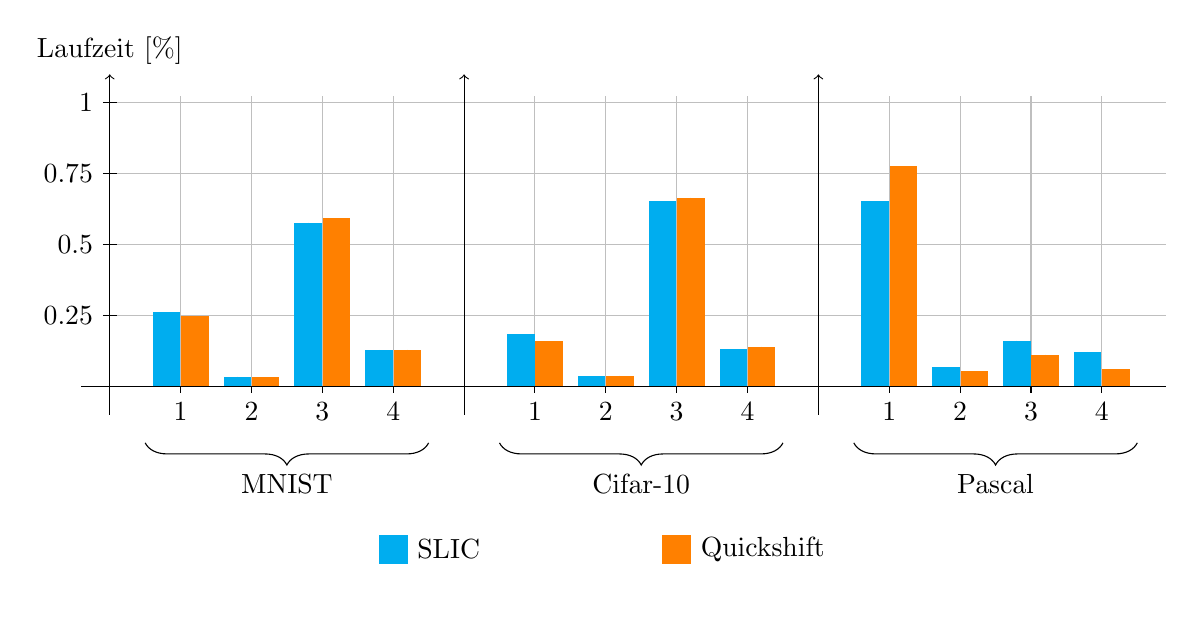
\begin{tikzpicture}[scale=0.9]
  \tikzstyle{slic}=[color=cyan, fill=cyan]
  \tikzstyle{quickshift}=[color=orange, fill=orange]

  \fill[white] (0, -2.9) rectangle (1, -1) node {};  % Abstand nach unten

  \draw[color=lightgray] (-0.1, -0.1) grid (14.9, 4.1);

  \draw[] (-0.4, 0) -- (14.9, 0);
  \draw[->] (0, -0.4) -- (0, 4.4) node[above] {Laufzeit [\%]};
  \draw[->] (5, -0.4) -- (5, 4.4);
  \draw[->] (10, -0.4) -- (10, 4.4);

  \draw (0.1, 1) -- (-0.1, 1) node[left] {$0.25$};
  \draw (0.1, 2) -- (-0.1, 2) node[left] {$0.5$};
  \draw (0.1, 3) -- (-0.1, 3) node[left] {$0.75$};
  \draw (0.1, 4) -- (-0.1, 4) node[left] {$1$};

  \draw[slic,       line width=0.35cm] (0.8, 0) -- (0.8, 1.0456);
  \draw[quickshift, line width=0.35cm] (1.2, 0) -- (1.2, 0.986);
  \draw (1, 0) -- (1, -0.1) node[below] {$1$};

  \draw[slic,       line width=0.35cm] (1.8, 0) -- (1.8, 0.1344);
  \draw[quickshift, line width=0.35cm] (2.2, 0) -- (2.2, 0.1224);
  \draw (2, 0) -- (2, -0.1) node[below] {$2$};

  \draw[slic,       line width=0.35cm] (2.8, 0) -- (2.8, 2.3084);
  \draw[quickshift, line width=0.35cm] (3.2, 0) -- (3.2, 2.3674);
  \draw (3, 0) -- (3, -0.1) node[below] {$3$};

  \draw[slic,       line width=0.35cm] (3.8, 0) -- (3.8, 0.5116);
  \draw[quickshift, line width=0.35cm] (4.2, 0) -- (4.2, 0.5148);
  \draw (4, 0) -- (4, -0.1) node[below] {$4$};

  \draw [decoration={brace,mirror,amplitude=8pt},decorate] (0.5,-0.8) -- node[below=8pt] {\gls{MNIST}} (4.5,-0.8);

  \draw[slic,       line width=0.35cm] (5.8, 0) -- (5.8, 0.7304);
  \draw[quickshift, line width=0.35cm] (6.2, 0) -- (6.2, 0.6336);
  \draw (6, 0) -- (6, -0.1) node[below] {$1$};

  \draw[slic,       line width=0.35cm] (6.8, 0) -- (6.8, 0.1388);
  \draw[quickshift, line width=0.35cm] (7.2, 0) -- (7.2, 0.1488);
  \draw (7, 0) -- (7, -0.1) node[below] {$2$};

  \draw[slic,       line width=0.35cm] (7.8, 0) -- (7.8, 2.61);
  \draw[quickshift, line width=0.35cm] (8.2, 0) -- (8.2, 2.6592);
  \draw (8, 0) -- (8, -0.1) node[below] {$3$};

  \draw[slic,       line width=0.35cm] (8.8, 0) -- (8.8, 0.5204);
  \draw[quickshift, line width=0.35cm] (9.2, 0) -- (9.2, 0.5584);
  \draw (9, 0) -- (9, -0.1) node[below] {$4$};

    \draw [decoration={brace,mirror,amplitude=8pt},decorate] (5.5,-0.8) -- node[below=8pt] {\gls{Cifar}-10} (9.5,-0.8);

  \draw[slic,       line width=0.35cm] (10.8, 0) -- (10.8, 2.6104);
  \draw[quickshift, line width=0.35cm] (11.2, 0) -- (11.2, 3.1044);
  \draw (11, 0) -- (11, -0.1) node[below] {$1$};

  \draw[slic,       line width=0.35cm] (11.8, 0) -- (11.8, 0.2636);
  \draw[quickshift, line width=0.35cm] (12.2, 0) -- (12.2, 0.2124);
  \draw (12, 0) -- (12, -0.1) node[below] {$2$};

  \draw[slic,       line width=0.35cm] (12.8, 0) -- (12.8, 0.6408);
  \draw[quickshift, line width=0.35cm] (13.2, 0) -- (13.2, 0.4432);
  \draw (13, 0) -- (13, -0.1) node[below] {$3$};

  \draw[slic,       line width=0.35cm] (13.8, 0) -- (13.8, 0.4852);
  \draw[quickshift, line width=0.35cm] (14.2, 0) -- (14.2, 0.24);
  \draw (14, 0) -- (14, -0.1) node[below] {$4$};

  \draw [decoration={brace,mirror,amplitude=8pt},decorate] (10.5,-0.8) -- node[below=8pt] {\gls{Pascal}} (14.5,-0.8);

  \tikzstyle{node}=[rectangle,draw, minimum width=10pt, minimum height=10pt, inner sep=0pt]
  \node[node, slic,       label=right:\gls{SLIC}] (1) at (4, -2.3) {};
  \node[node, quickshift, label=right:Quickshift] (2) at (8, -2.3) {};
\end{tikzpicture}

\begin{tabular}{ll}
  \toprule
  1. Segmentierung & 2. Adjazenzbestimmung\\
  3. Graphvergröberung (4 Ebenen) & 4. Merkmalsextraktion\\
  \bottomrule
\end{tabular}

\caption[Laufzeitverteilung der spektralen Vorverarbeitungsschritte]{Laufzeitverteilung der einzelnen Vorverarbeitungsschritte für das spektrale Lernen auf Graphen, unterteilt \bzgl{} unterschiedlichen Datensätze \gls{MNIST}, \gls{Cifar}-10 und \gls{Pascal} und den verwendeteten Superpixelalgorithmen \gls{SLIC} und Quickshift.
Wohingegen für \gls{MNIST} und \gls{Cifar}-10 die Graphvergröberung die längste Berechnungsdauer in Anspruch nimmt, zeigt sich dagegegen für größere Datensätze (\gls{Pascal}) die Segmentierung als Flaschenhals der Vorverarbeitung.}
\label{fig:laufzeit_spektral_pipeline}
\end{figure}

Anstelle der Receptive-Field-Berechnung entsteht hier ein Mehraufwand durch die Berechnung der Graphvergröberung.
Dieser Aufwand zeigt sich jedoch auf Bildern aus \gls{Pascal} als zu vernachlässigen, da die Laufzeit bei großen Bildern (fast) rein von der Laufzeit der Superpixelalgorithmen abhängig ist.

Tabelle~\ref{tab:laufzeit_raeumlich_spektral} stellt die absoluten Aufwände zur räumlichen sowie spektralen Vorverarbeitung eines Bildes aus allen Datensätze und Superpixelalgorithmen gegenüber.
\begin{table}[t]
\centering
\begin{tabular}{lrrrr}
  \toprule
  & \multicolumn{2}{c}{Räumlich [ms]} & \multicolumn{2}{c}{Spektral [ms]}\\
  \cmidrule{2-5}
  & \acs{SLIC} & \acs{QS} & \acs{SLIC} & \acs{QS}\\
  \midrule
  \acs{MNIST} & 30.59 & 24.00 & 20.32 & 19.40\\
  \acs{Cifar}-10 & 72.74 & 43.85 & 25.34 & 23.18\\
  \acs{Pascal} & 713.40 & 1080.78 & 372.79 & 782.56\\
  \bottomrule
\end{tabular}
\caption[Laufzeiten der räumlichen und spektralen Vorverarbeitung]{Laufzeiten der räumlichen sowie spektralen Vorverarbeitung für ein Bild der jeweiligen Datensätze und Superpixelalgorithmen basierend auf den Laufzeiten aus Abbildung~\ref{fig:laufzeit_raeumlich_pipeline} und~\ref{fig:laufzeit_spektral_pipeline}.
Die räumliche Vorverarbeitung ist aufgrund der einzelnen Receptive-Field-Berechnungen deutlich ineffizienter.}
\label{tab:laufzeit_raeumlich_spektral}
\end{table}
Wohingegen sich für Bilder mit kleinen Auflösungen aus den Datensätzen \gls{MNIST} und \gls{Cifar}-10 der Aufwand zur Vorverarbeitung in Grenzen hält, zeigen sich für ein Bild aus \gls{Pascal} die Kosten zur Vorverarbeitung als nicht zu unterschätzen.
Eine Vorverarbeitung zur Laufzeit ist auf diesem Datensatz daher (zurzeit) nicht zu empfehlen.
Weiterhin sei anzumerken, dass die spektralen Vorverarbeitungsschritte in jedem Versuchsaufbau entschieden schneller als die räumlichen berechnet werden können.

\paragraph{Training}

Tabelle~\ref{tab:train_laufzeit} zeigt die im Durschnitt ermittelten Laufzeiten des Trainings eines Batches der Größe $64$ für alle vorgestellten Netzarchitekturen.
\begin{table}[t]
\centering
\resizebox{\textwidth}{!}{%
\begin{tabular}{lllrrrr}
  \toprule
  Datensatz & Superpixel & Verfahren & \multicolumn{4}{c}{Laufzeit [s]}\\
  \cmidrule{4-7}
   & & & vor Beginn & \multicolumn{3}{c}{zur Laufzeit}\\
  \cmidrule{5-7}
   & & & & Vorverarbeitung & Training & $\sum$\\
  \midrule
  \gls{MNIST} & \gls{SLIC} & \acs{RL} & 0.04 & \multicolumn{3}{c}{—}\\
  \gls{MNIST} & \gls{SLIC} & \acs{SGCNN} & & \multicolumn{3}{c}{—}\\
  \gls{MNIST} & \gls{SLIC} & \acs{GCN} & 0.20 & \multicolumn{3}{c}{—}\\
  \gls{MNIST} & \gls{SLIC} & \acs{EGCNN} & 0.61 & \multicolumn{3}{c}{—}\\
  \gls{MNIST} & \acs{QS}   & \acs{RL} & 0.04 & \multicolumn{3}{c}{—}\\
  \gls{MNIST} & \acs{QS}   & \acs{SGCNN} & 0.37 & \multicolumn{3}{c}{—}\\
  \gls{MNIST} & \acs{QS}   & \acs{GCN} & 0.21 & \multicolumn{3}{c}{—}\\
  \gls{MNIST} & \acs{QS}   & \acs{EGCNN} & 0.63 & \multicolumn{3}{c}{—}\\
  \midrule
  \gls{Cifar}-10 & \gls{SLIC} & \acs{SGCNN} & — & & & \\
  \gls{Cifar}-10 & \gls{SLIC} & \acs{GCN} &   — & 1.24 & 0.39 & 1.63 \\
  \gls{Cifar}-10 & \gls{SLIC} & \acs{EGCNN} & — & 0.44 & 2.00 & 2.44 \\
  \gls{Cifar}-10 & \acs{QS}   & \acs{SGCNN} & — & 0.43 & 1.95 & 2.38\\
  \gls{Cifar}-10 & \acs{QS}   & \acs{GCN} &   — & 1.09 & 0.36 & 1.45\\
  \gls{Cifar}-10 & \acs{QS}   & \acs{EGCNN} & — & & & \\
  \midrule
  \gls{Pascal} & \gls{SLIC} & \acs{EGCNN} & & 23.05 & 4.17 & 27.22\\
  \gls{Pascal} & \acs{QS}   & \acs{EGCNN} & 5.28 & 51.32 & 5.46 & 56.78 \\
  \midrule
  \gls{MNIST} & — & klassisch & & \multicolumn{3}{c}{—}\\
  \gls{Cifar}-10 & — & klassisch & 0.49 & \multicolumn{3}{c}{—}\\
  \gls{Pascal} & — & klassisch & & \multicolumn{3}{c}{—}\\
  \bottomrule
\end{tabular}}
\caption[Vergleich der Trainingslaufzeiten]{Vergleich der Laufzeiten des Trainings eines Batches der Größe 64 für alle vorgestellten Netzarchitekturen.}
\label{tab:train_laufzeit}
\end{table}
Die Eingabedaten wurden für \gls{MNIST} \bzw{} \gls{Pascal} aufgrund nicht benötigter Augmentierung \bzw{} der aufwändigen Berechnungen vorab gespeichert, wohingegen die Grapheingabedaten für \gls{Cifar}-10 zur Laufzeit generiert wurden.
Es zeigt sich, dass das Training auf Graphen im Allgemeinen deutlich langsamer als im Vergleich zu ausgereiften Bildimplementierungen ist.
Lediglich der Ansatz des räumlichen Lernens kann aufgrund seiner Verwendung der klassischen Faltungsoperation und bei einer Vorverarbeitung vor Beginn des Trainings schnelle Laufzeiten garantieren.

Zwischen den spektralen Faltungsansätzen zeigt sich das \acs{GCN} aufgrund seiner geringen Berechnungskomplexität als sehr effizient, leidet jedoch wie in Kapitel~\ref{ergebnisse} beschrieben an mangelnder Genauigkeit.
Das \acs{EGCNN} weist unter allen Ansätzen die höchste Berechnungskomplexität auf.
Dies ist im Vergleich mit dem \acs{SGCNN} insoweit zu erklären, dass dessen Netzarchitektur in der Regel tiefer ist und mehrere Faltungsschichten hintereinander verlangt, um an Informationen nicht direkt benachbarter Knoten zu gelangen.
Das \acs{SGCNN} erfordert dies nicht, da dessen Filtergröße in direktem Zusammenhang zur Größe der Faltung steht.

Es ist weiter bei einer Vorverarbeitung während des Trainings zu beobachten, dass die Aufwände für die Vorverarbeitung umso höher werden, umso schneller die eigentliche Lernprozedur vonstatten geht.
So zeigt sich \bspw{} bei \gls{Cifar}-10, dass das \acs{EGCNN} und \acs{SGCNN} in der Regel lediglich $\approx$ 0.4s auf die Vorverarbeitung warten müssen, wohingegen bei der effizienteren Faltung des \acs{GCN}s das Training pro Batch $\approx$ 1.1s pausiert.
Damit wird trotz Multithreading die Vorverarbeitung zur Laufzeit zum Flaschenhals des Trainings.

\paragraph{Vergleich \bzgl{} vorhandener Implementierungen}
\label{vergleich_laufzeit}

Obwohl die Vorverarbeitung das Training eines neuronalen Netzes zur Laufzeit behindern kann, so konnten bereits viele Vorverarbeitungsschritte im Laufe dieser Arbeit effizienter als ihre vorhandenen, quelloffenenen Implementierungen gestaltet werden.
So besitzt \bspw{} \texttt{skimage} eine Implementierung zur Adjazenzbestimmung einer Segmentierungsmaske und zur Extraktion der meisten in dieser Arbeit vorgestellten Merkmale.
Beide Verfahren konnten mit deutlichem Laufzeitgewinnn optimiert werden.
Der frei zugängliche Quelltext des spektralen Faltungsoperators (\acs{SGCNN}) besitzt ebenso eine Implementierung zur Vergröberung eines Graphen.
Dieser konnte, trotz der Berücksichtigung der Knotenpositionen und Generierung zweier Adjazenzmatrizen \gls{Adist} und \gls{Arad}, fast dreimal so schnell implementiert werden.
Abbildung~\ref{fig:laufzeit_vergleich} fasst die beschriebenen Laufzeitgewinne separat zusammen.
\begin{figure}[t]
\centering
  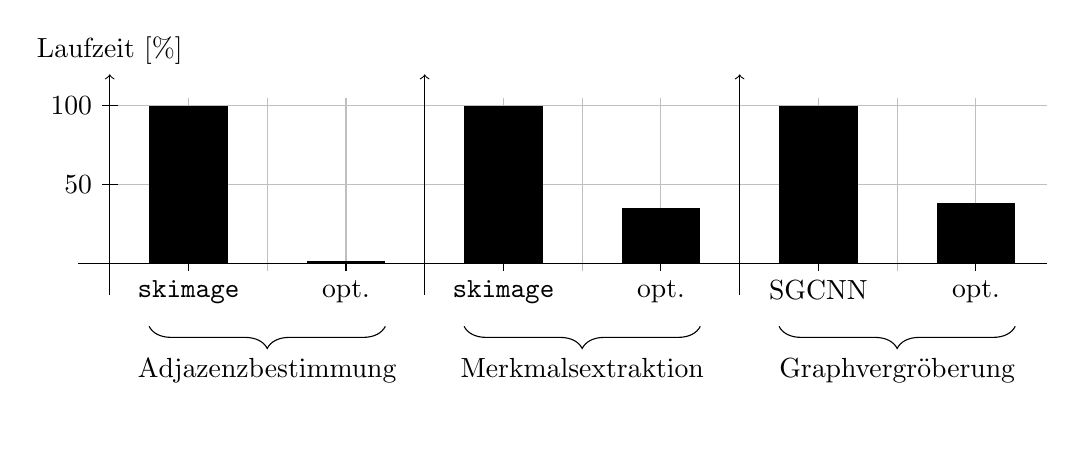
\begin{tikzpicture}[]
  \fill[white] (0, -2) rectangle (1, -1) node {};  % Abstand nach unten

  \draw[color=lightgray] (-0.1, -0.1) grid (11.9, 2.1);

  \draw[] (-0.4, 0) -- (11.9, 0);
  \draw[->] (0, -0.4) -- (0, 2.4) node[above] {Laufzeit [\%]};
  \draw[->] (4, -0.4) -- (4, 2.4);
  \draw[->] (8, -0.4) -- (8, 2.4);

  \draw (0.1, 1) -- (-0.1, 1) node[left] {$50$};
  \draw (0.1, 2) -- (-0.1, 2) node[left] {$100$};

  \draw[line width=1cm] (1, 0) -- (1, 2);
  \draw[line width=1cm] (3, 0) -- (3, 0.030153);
  \draw (1, 0) -- (1, -0.1) node[below] {\texttt{skimage}};
  \draw (3, 0) -- (3, -0.1) node[below] {opt.};
  \draw [decoration={brace,mirror,amplitude=8pt},decorate] (0.5,-0.8) -- node[below=8pt] {Adjazenzbestimmung} (3.5,-0.8);

  \draw[line width=1cm] (5, 0) -- (5, 2);
  \draw[line width=1cm] (7, 0) -- (7, 0.704036);
  \draw (5, 0) -- (5, -0.1)  node[below] {\texttt{skimage}};
  \draw (7, 0) -- (7,  -0.1) node[below] {opt.};
  \draw [decoration={brace,mirror,amplitude=8pt},decorate] (4.5,-0.8) -- node[below=8pt] {Merkmalsextraktion} (7.5,-0.8);

  \draw[line width=1cm] (9, 0)   -- (9, 2);
  \draw[line width=1cm] (11,  0) -- (11,  0.769867);
  \draw (9, 0)  -- (9, -0.1)  node[below] {\acs{SGCNN}};
  \draw (11, 0) -- (11, -0.1) node[below] {opt.};
  \draw [decoration={brace,mirror,amplitude=8pt},decorate] (8.5,-0.8) -- node[below=8pt] {Graphvergröberung} (11.5,-0.8);

\end{tikzpicture}

\begin{tabular}{lrrr}
  \toprule
  Vorverarbeitungsschritt & vorhanden [ms] & optimiert [ms] & Gewinn [\%]\\
  \midrule
  Adjazenzbestimmung & 866 & 13 & 6615\\
  Merkmalsextraktion & 144 & 50 & 288\\
  Graphvergröberung (4 Ebenen) & 87 & 33 & 264\\
  \bottomrule
\end{tabular}

\caption[Laufzeitvergleich \bzgl{} anderer Implementierungen]{Vergleich der Laufzeiten verschiedener Vorverarbeitungsschritte \bzgl{} des Lernens auf Graphen zwischen bereits vorhandenen, quelloffenen Implementierungen (links) und ihren jeweiligen entwickelten optimierten Versionen (rechts) am Beispiel eines Bildes aus \gls{Pascal}: (1) Adjazenzbestimmung einer Segmentierungsmaske, (2) Merkmalsextraktion und (3) Graphvergröberung inklusive der entsprechenden Anordung der Knoten zu binären Bäumen.
  In allen Bereichen konnten deutliche Laufzeitgewinne erreicht werden.}
\label{fig:laufzeit_vergleich}
\end{figure}

